
\documentclass[tikz]{standalone} % this expands the doc to contain all drawings.
\usetikzlibrary{lindenmayersystems}

\tikzset{
  Koch curve/.style = {
    l-system={
      rule set={F -> F-F++F-F},
      axiom=F++F++F,
      step=1pt,
      angle=60,
      #1
    }
  }
}

\begin{document}
This is a very long sentence. This is a very long sentence. This is a very long sentence.
This is a very long sentence. This is a very long sentence. This is a very long sentence.
\begin{tikzpicture} % to put all pictures in one big picture
    \node (a) at (0,0) {
      \begin{tikzpicture}
      \draw[Koch curve={order=0,step=100pt}] l-system -- cycle;
      \end{tikzpicture}
    };

    \node (b) at (a.east) [anchor=west, xshift=1cm]{ % move right by 2cm
        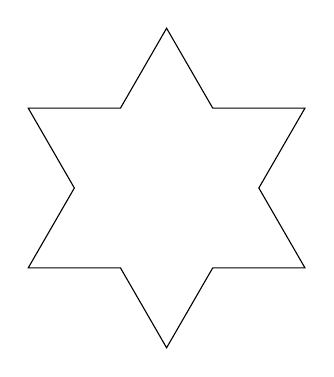
\begin{tikzpicture}
        \draw[Koch curve={order=1,step=100pt/3}] l-system -- cycle;
        \end{tikzpicture}
    };

    \node (c) at (b.east) [anchor=west, xshift=1cm]{
        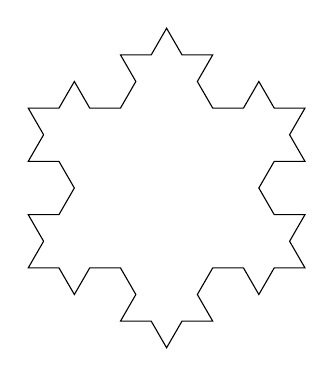
\begin{tikzpicture}
        \draw[Koch curve={order=2,step=100pt/(3^2)}] l-system -- cycle;
        \end{tikzpicture}
    };

    \node (d) at (c.east) [anchor=west, xshift=1cm]{
        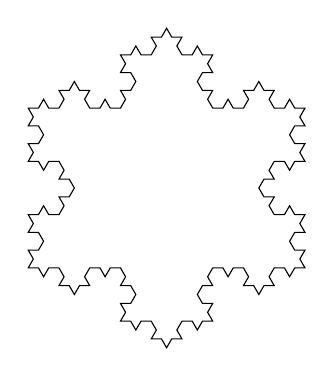
\begin{tikzpicture}
        \draw[Koch curve={order=3,step=100pt/(3^3)}] l-system -- cycle;
        \end{tikzpicture}
    };
\end{tikzpicture}

\end{document}
